\documentclass{article}
\usepackage{amsmath,amssymb,amsthm}
\usepackage{enumerate}
\usepackage{mathtools}
\usepackage{graphicx}
\usepackage{caption}
\newtheorem{theorem}{Theorem}
\newtheorem{question}[theorem]{Question}
\newtheorem{answer}[theorem]{Solution}
\begin{document}
\begin{question}
	Show that the vectors $\begin{pmatrix} 
		 +2\\-1\\+1 
	\end{pmatrix}$, $\begin{pmatrix} 
	 +1\\-3\\-5 
\end{pmatrix}$ and $\begin{pmatrix} 
+3\\-4\\-4 
\end{pmatrix}$ form the vertices of a right angled trianle.
\end{question}
Solution. Let $A$, $B$ and $C$ be given vectors such that $A =\begin{pmatrix} 
	+2\\-1\\+1 
\end{pmatrix}$,\\     
$B= \begin{pmatrix} 
+1\\-3\\-5 
\end{pmatrix}$ and $C= \begin{pmatrix} 
+3\\-4\\-4 
\end{pmatrix}$.\\
To show that $A$, $B$ and $C$ form the vertices of a right angled triangle. First we need to show that $A$, $B$ and $C$ are indeed vertices of a triangle.\\
For this we need to see if the vertices satisfy triangle inequality. Let $a$, $b$ and $c$ denote the length of vectors $\overrightarrow{A-B}$, $\overrightarrow{B-C}$ and $\overrightarrow{C-A}$. Now,\\
$a=\sqrt{41}$, $b=\sqrt{6}$ and $c=\sqrt{35}$. We can see that  $a+b>c$, 
$a+c>b$ and $b+c >a$. Thus, the given vectors $A$, $B$ and $C$ form the vertices of a triangle.\\


 \begin{figure}[!htb]
	\center{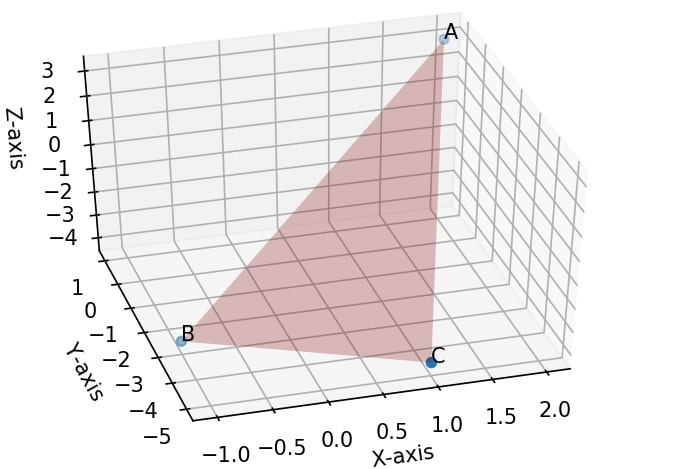
\includegraphics[width=\textwidth]
		{assignment1fig-1.jpg}}
	\caption{\label{fig1}}
\end{figure}

To prove, the $\triangle ABC$ is a right triangle, we need to calculate the inner product of all the below vectors and check if any one of them is 0.:
\begin{enumerate}[1.]
	\item $\langle \overrightarrow{A-C}  ,\overrightarrow{B-C}\rangle$ = $\overrightarrow{(A-C)}^T$ $\overrightarrow{(B-C)}$ = $(-1\;\; 3 \;\; 5)$ $\begin{pmatrix} 
		-2\\+1\\-1 
	\end{pmatrix}$ = 0
\end{enumerate}
\begin{enumerate}[2.]
	\item $\langle \overrightarrow{A-B}  ,\overrightarrow{C-B}\rangle$ = $\overrightarrow{(A-B)}^T$ $\overrightarrow{(C-B)}$ = $(1\;\; 2 \;\; 6)$ $\begin{pmatrix} 
		+2\\-1\\+1 
	\end{pmatrix}$ = 6
\end{enumerate}

\begin{enumerate}[3.]
	\item $\langle \overrightarrow{B-A}  ,\overrightarrow{C-A}\rangle$ = $\overrightarrow{(B-A)}^T$ $\overrightarrow{(C-A)}$ = $(-1\;\; -2 \;\; -6)$ $\begin{pmatrix} 
		+1\\-3\\-5 
	\end{pmatrix}$ = 35
\end{enumerate}
Clearly, from $(1).$ we can see that $\triangle$ABC is right angled at C.
\end{document}
